\documentclass[twocolumn]{article}

\usepackage{scrextend}
\changefontsizes{8pt}

\makeatletter
\renewcommand*{\fps@figure}{!htb}
\renewcommand*{\fps@table}{!htb}
\makeatother

\usepackage{sectsty}
\sectionfont{\fontsize{11}{11}\selectfont}
\subsectionfont{\fontsize{10}{11}\selectfont}

% \usepackage[compact]{titlesec}
% \titlespacing{\section}{0pt}{2ex}{1ex}
% \titlespacing{\subsection}{0pt}{1ex}{1ex}
% \titlespacing{\subsubsection}{0pt}{0.5ex}{1ex}

\setlength{\parskip}{0cm}
\setlength{\parindent}{1em}

\usepackage{geometry}
 \geometry{
 a4paper,
 total={170mm,257mm},
 left=20mm,
 top=20mm,
 }
\usepackage[utf8]{inputenc}
\usepackage[hidelinks]{hyperref}
\usepackage{amsmath, bm}
\usepackage[ruled,vlined]{algorithm2e}
\usepackage{amssymb}
\usepackage{graphicx}
\usepackage{float}
\usepackage{booktabs}
\usepackage[parfill]{parskip}
\usepackage{comment}
\usepackage{subcaption}
\usepackage{booktabs}



\usepackage{listings}
\lstset{
    language=Python,
    breaklines=true,
    breakatwhitespace=true,
    basicstyle=\footnotesize,
    frame=lines
}
\usepackage[capitalise, nameinlink]{cleveref}

\usepackage[sorting=none, style=verbose]{biblatex}
\addbibresource{lab_5.bib}

\usepackage{titling}
\setlength{\droptitle}{-1cm}

\title{\Large COMP6248 Lab 5 Exercise -- A little Linear Regression}
\author{\small Wei Chien Teoh (Eugene)\\\bigskip \href{mailto:wct1c16@soton.ac.uk}{wct1c16@soton.ac.uk}}
\date{\small 29 April 2021}

\begin{document}

\maketitle

\section*{Introduction}

The results are seeded using \lstinline{pytorch_lightning.seed_everything(0)} to provide reproducible results. All plots are generated using Weights \& Biases \autocite{WeightsBiases}.

\section{An initial attempt} \label{sec:1}

\subsection{A simple CNN baseline}

The image-to-vector regression task given is described as a regression problem, thus the Mean Squared Error (MSE) loss function will be used for all models in this exercise. The goal is to predict the coefficients of the regression lines from the images.

The learning curves and performance of all models is illustrated in \cref{fig:train-loss,fig:val-loss,fig:test-loss}. \cref{tab:properties} shows more properties for the models. Models 1 to 3 corresponds to the models built in \cref{sec:1,sec:2,sec:3}.

Model 1 provides the best training performance but gives a high validation and test loss relative to it's training. This is possibly due to the large complexity of the model, 9.8 M parameters. The model is likely overfitting on the training data.


\section{A second attempt} \label{sec:2}

\subsection{A simple CNN with global pooling}

Model 2 provides the worse performances for all train, validation and test loss. This is due to the lower complexity of the model. However, all the losses is relatively close, thus we can conclude that it generalises well to the validation and test set. A benefit of Model 2 is the shorter training time compared to Model 1.


\section{Something that actually works?} \label{sec:3}

\subsection{Let's regress}

Model 3 improves on previous models by adding two interleaved channels of equally spaced values ranging from -5 to 5. The third channel is the transpose/rotation of the second. The original data channel is sparse. The interleaved channels provide a form of data augmentation that allows the convolutional layers to better learn the structure of the original sparse data.

By introducing the interleaved channels, Model 3 outperforms Model 2 in training loss and Model 1 in validation loss. It also significantly outperforms the previous models in test loss. Hence, it can be concluded that Model 3 provides the best generalisation out of all the models. The training time is reasonable relative to the previous models as the model complexity is similar to Model 2.

\begin{figure}
    \centering
    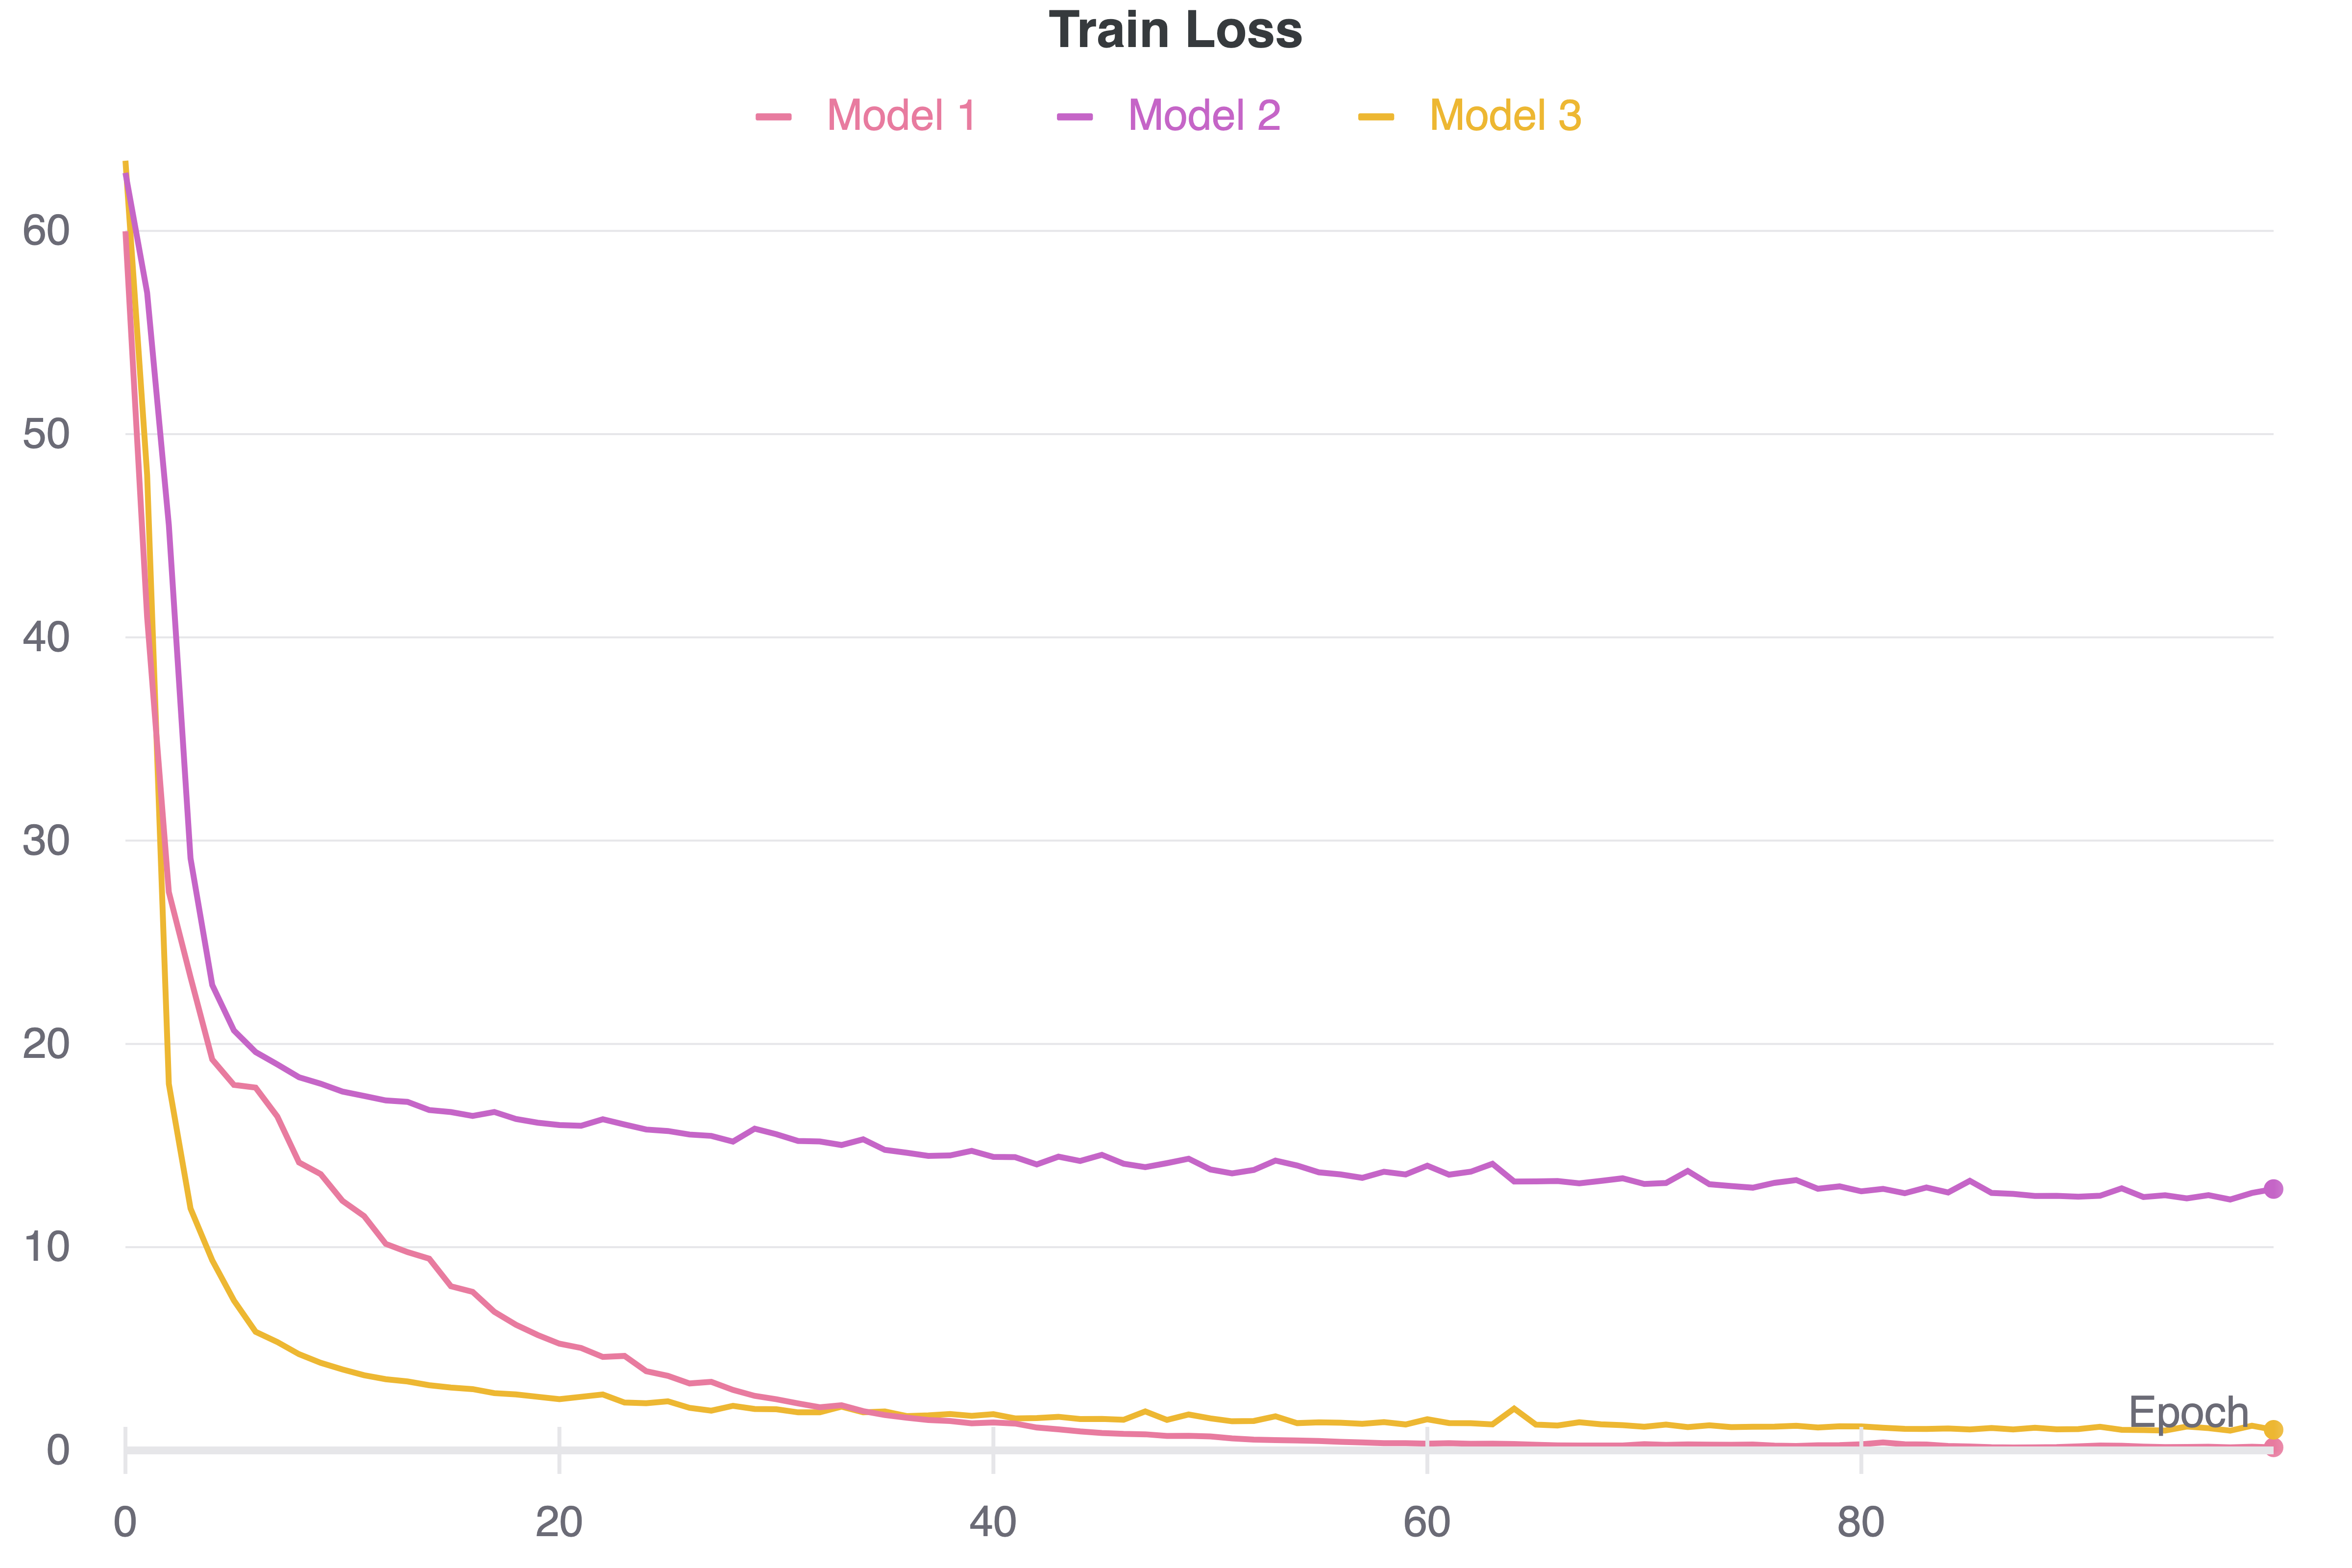
\includegraphics[width=\linewidth]{Figures/train-loss.png}
    \caption{Train loss. Final values: (1) 0.149 (2) 12.859 (3) 1.013.}
    \label{fig:train-loss}
\end{figure}

\begin{figure}
    \centering
    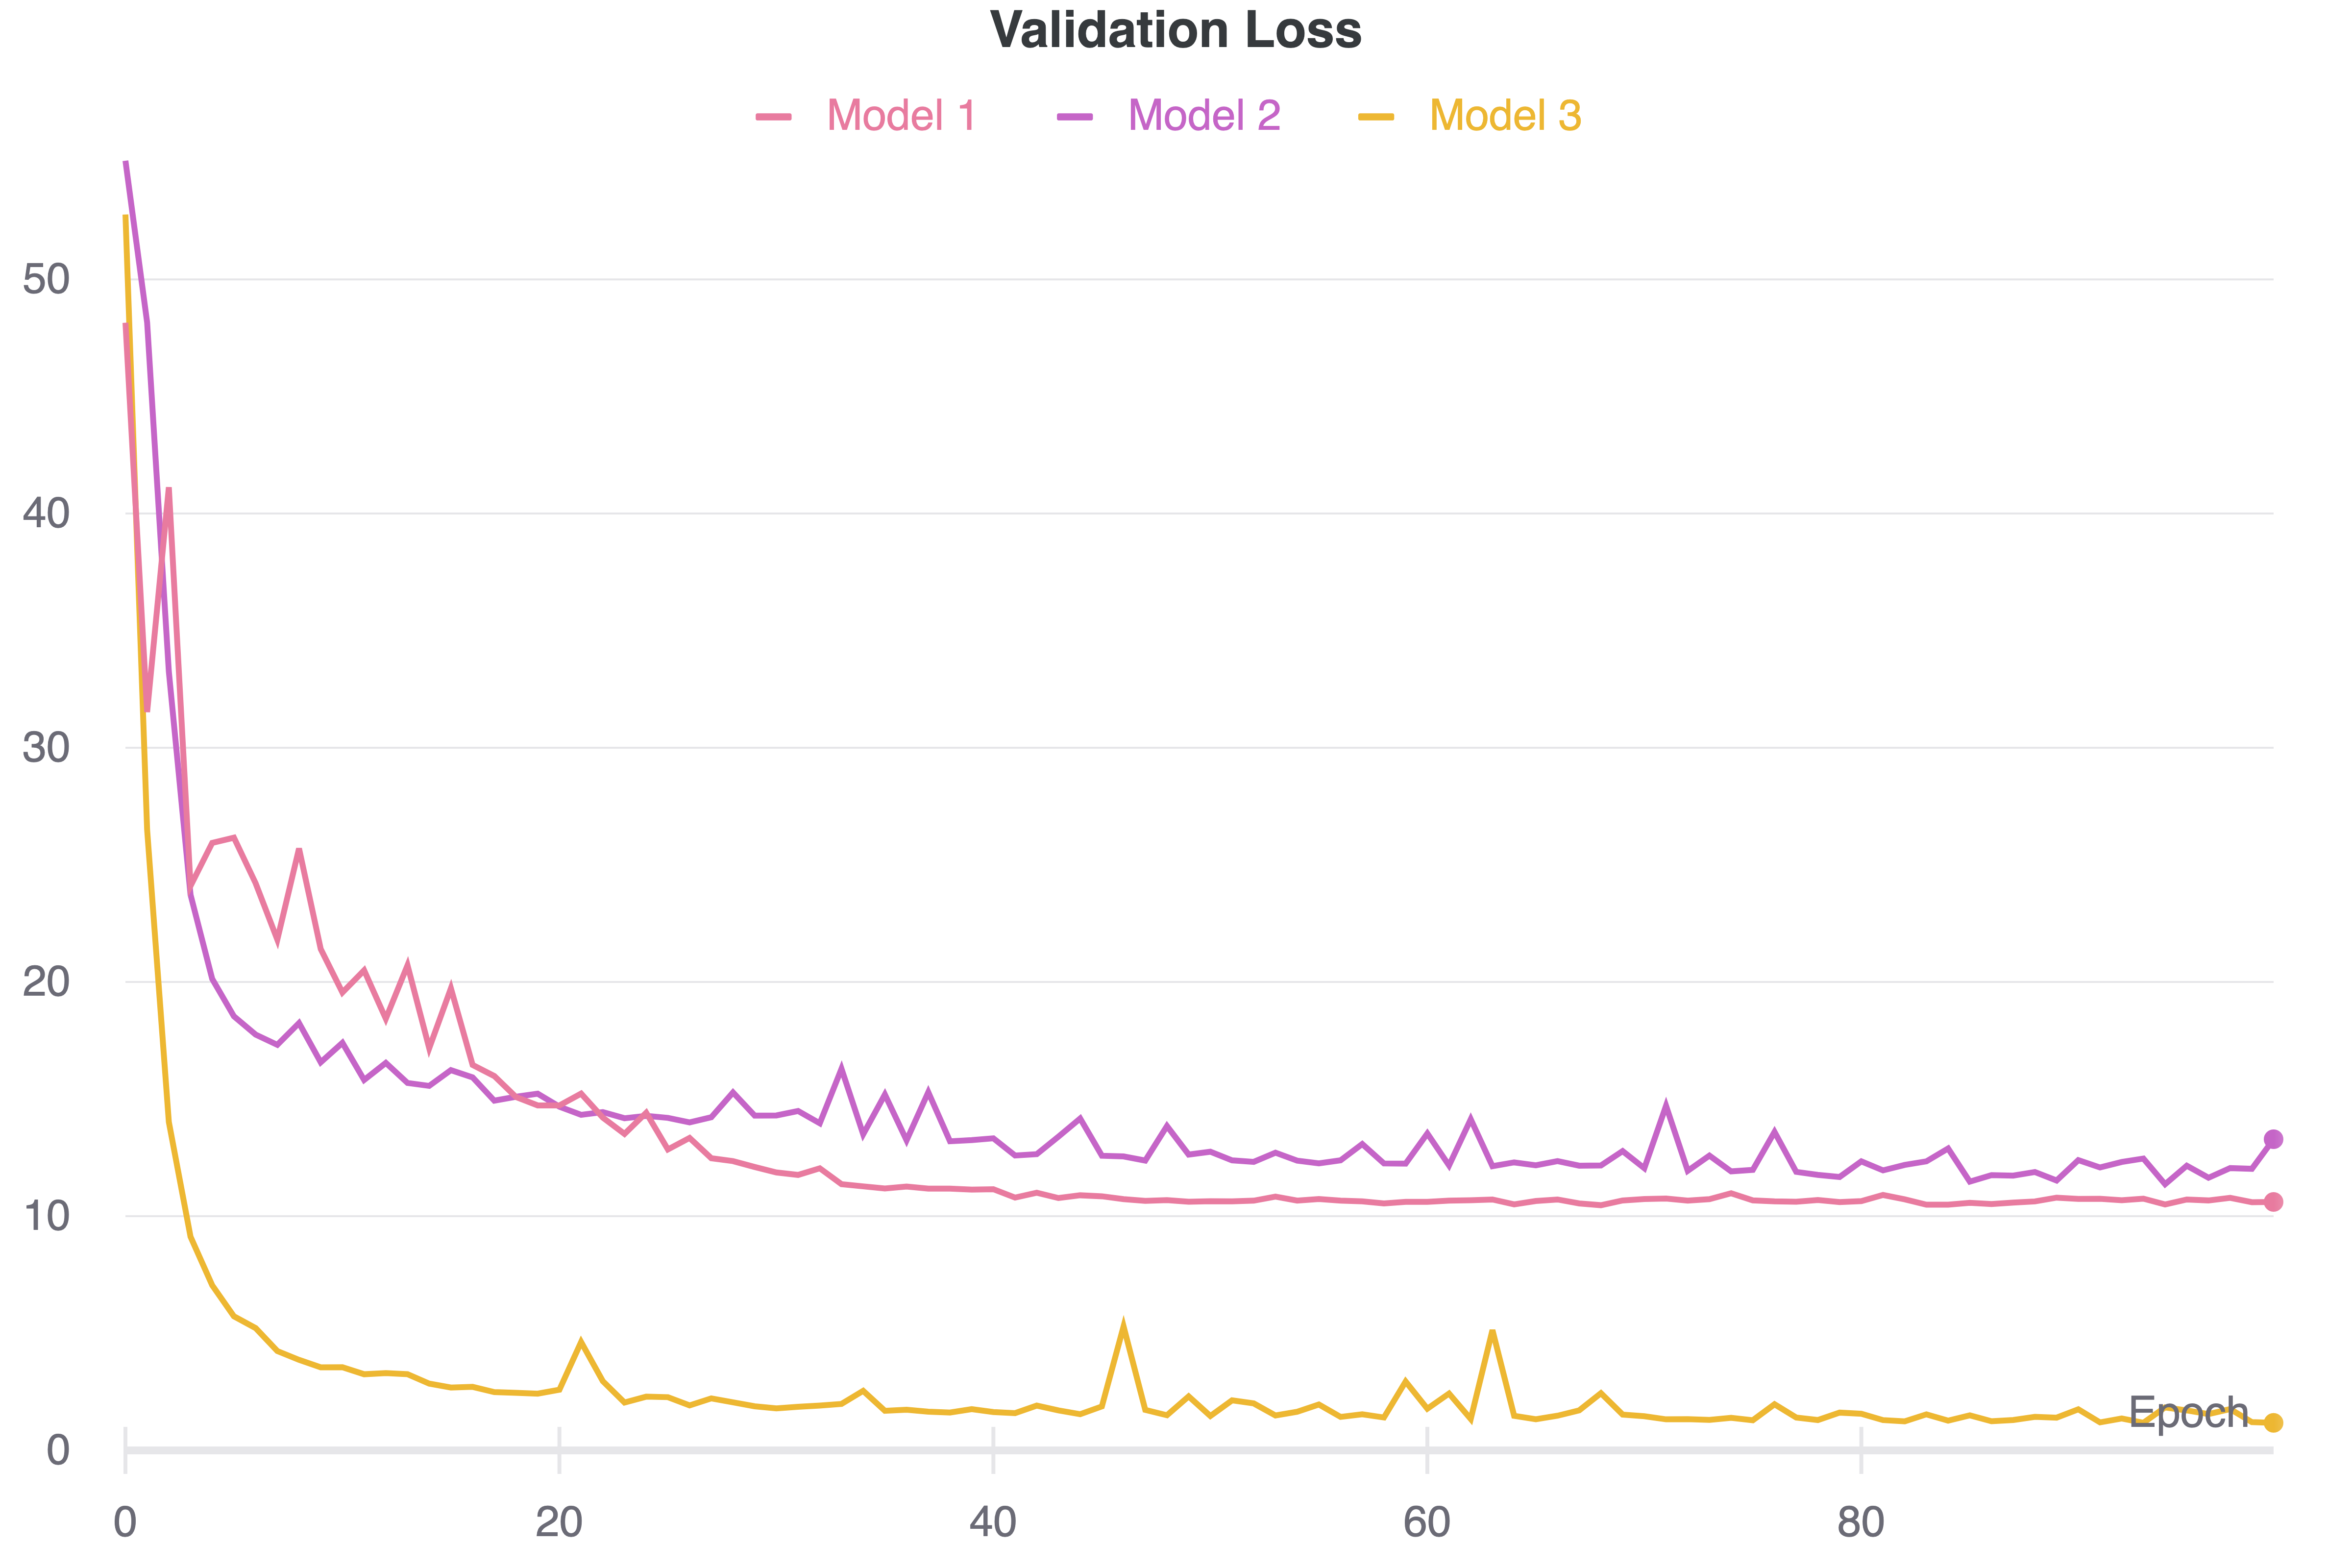
\includegraphics[width=\linewidth]{Figures/val-loss.png}
    \caption{Validation loss. (1) 10.608 (2) 13.287 (3) 1.176.}
    \label{fig:val-loss}
\end{figure}

\begin{figure}
    \centering
    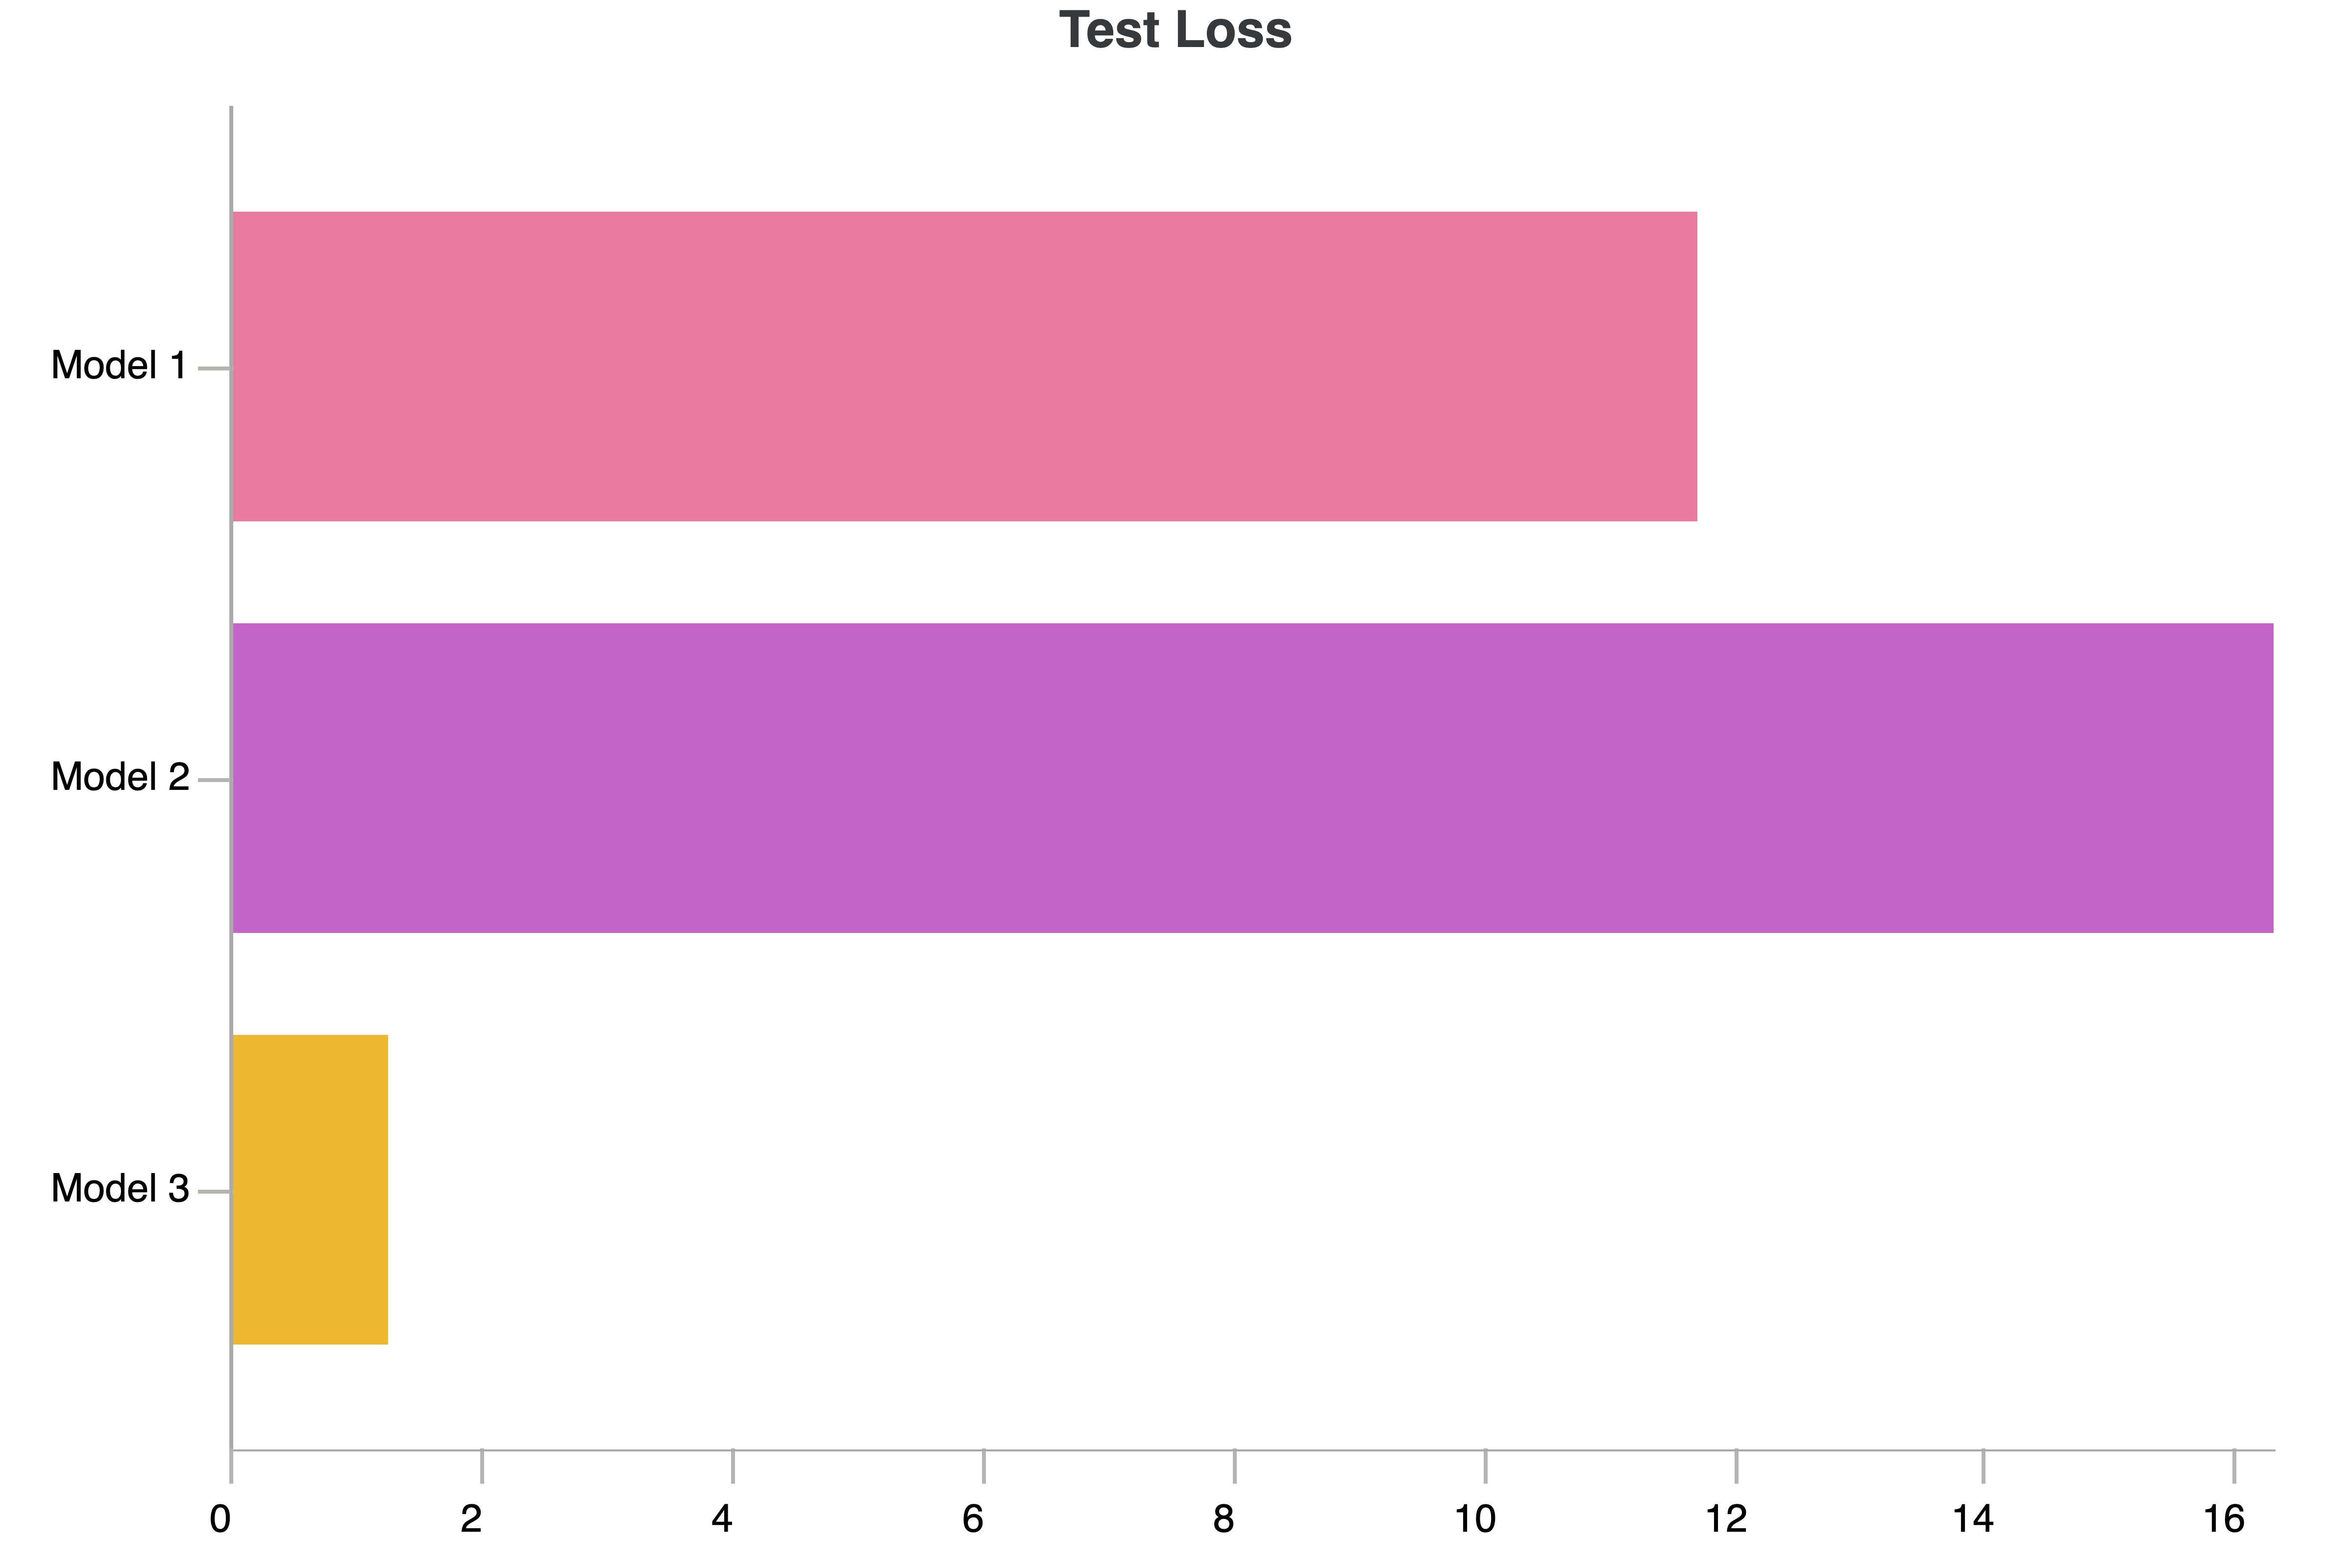
\includegraphics[width=\linewidth]{Figures/test-loss.png}
    \caption{Test loss. (1) 11.697 (2) 16.302 (3) 1.236.}
    \label{fig:test-loss}
\end{figure}

\begin{table}
    \centering
    \caption{Runtime and total parameters.}
    \label{tab:properties}
    \begin{tabular}{lrl}
    \toprule
    Model &         Runtime & Total Parameters \\
    \midrule
    1 & 7m 13s &            9.8 M \\
    2 & 4m 50s &           27.8 K \\
    3 & 4m 52s &           28.7 K \\
    \bottomrule
    \end{tabular}
    \end{table}


\end{document}